\section{Processor Optimizations}
\label{sec:processor_opt}

Our processor optimizations are based on arithmetic operations, such as addition and multiplication, which are performance critical in training computations, and have predetermined results when one of the input operands is a zero. We refer to machine instructions that perform such arithmetic operations as ``zero-optimizable'' instructions. Exploiting zero-optimizable instructions to improve training peformance is promising because, as shown in our profiling studies (Figure~\ref{fig:cifar-10_word_sparsity}), a significant portion of the inputs to training computations are zeroes. 

\begin{comment}
\begin{figure}
\centering

\includegraphics[height=1.4in, width=.9\columnwidth]{Figures/gradient_machine_code.png}
\caption{(a) original and (b) optimized machine code of the inner loop for computing weight deltas.}
\label{fig:deltas_code_opt}
\end{figure}
\end{comment}

\begin{figure*}
\centering

\includegraphics[height=1.4in, width=1.9\columnwidth]{Figures/deltas_code_opt.png}
\caption{(a) Deltas computation inner loop;  optimized for R$2$ is zero in (b) one and (c) $N$ iterations; (d) for R$1$ is zero.}
\label{fig:deltas_code_opt}
\end{figure*}


\subsection{Opportunities}

We discuss the dynamic optimization opportunities that motivate our processor techniques using the machine code sequences in Figure~\ref{fig:deltas_code_opt}, which correspond to the inner loop of the gradient computation code in Figure~\ref{fig:deltas_source_code}.    Figure~\ref{fig:deltas_code_opt}(a) represents machine code of the loop\footnote{Our example in Figure~\ref{fig:deltas_code_opt} is unoptimized for simplicity of explanation.}, and includes five zero-optimizable instructions: I$3$, I$4$, I$6$, I$7$, and I$8$.  
R$1$ corresponds to the loop invariant \emph{errors[j]}, the R$2$ target of I$1$ corresponds to \emph{activations[i]}, and R$4$ target of I$2$ corresponds to \emph{deltas[k]} of the code snippet in Figure~\ref{fig:deltas_source_code}.

\subsubsection{Zero-Optimizable Instructions.} A zero-optimizable instruction presents a number of opportunities to increase ILP and reduce resource pressure of training workloads on modern out-of-order processors.  These opportunities arise because of the predetermined results of zero-optimizable instructions when computing on zero input operands.  Since our focus is on zero-optimizable instructions which perform additions or multiplications, we examine the effect of a zero input operand when the instructions have two input operands, and an input operand is also the output operand. 

A zero input operand converts an addition instruction into a copy operation of the other input operand into the destination location. Also, if the other input operand is also the destination operand then the copy operation is redundant.  For multiplications, a zero input operand results in a zero value of the destination operand regardless of the value of the other input operand.  Thus, zero input operands can make some data dependencies and pipeline stages redundant for zero-optimizable and dependent instructions.  Consequently, zero-optimizable and dependent instructions can be issued or commited earlier than normal or eliminated completely, as discussed below. 

\subsubsection{Early Instruction Issue/Commit.}  Normally, an instruction cannot be issued to the execution stage until both input operands are available. However, a multiplication instruction can be issued immediately an input operand is available as zero since the result (i.e., zero) is now independent of the other operand.  For example, I$3$ can be issued once R$1$ is discovered to be zero without waiting for load I$2$ to complete; I$3$ becomes independent of I$2$.  Moreover, I$3$ can proceed to the commit stage, bypassing the multiplication functional unit, because the result and side effect (set R$2$ to zero)  can be directly generated.  Early issue and commit of zero-optimizable instructions can reduce pipeline resource pressure and the waiting times of data dependent instructions, (e.g., I$4$), since those dependences are satisfied quicker. 

\begin{comment}
\begin{figure}
\centering
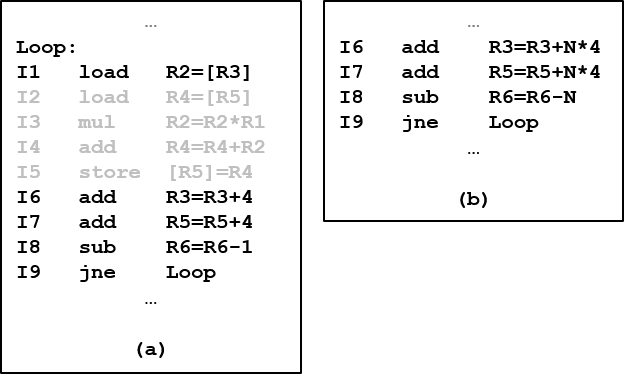
\includegraphics[height=1.4in, width=.9\columnwidth]{Figures/r2_deltas_opts.png}
\caption{Loop optimizations if R2 is zero for (a) one iteration (dead instructions are grey), and (b) $N$ consecutive iterations.}
\label{fig:r2_deltas_opts}
\end{figure}
\end{comment}

\subsubsection{Dead Instruction Elimination.} A zero input can make a zero-optimizable instruction redundant (or dead), and safe to eliminate from execution, as well as instructions which it depends on (producers) or which depend on it (consumers).  We exploit this property to improve performance by executing optimized versions of loops, without dead instructions, when a zero-optimizable instruction input is zero.  For concreteness, we examine the opportunities to eliminate dead instructions in loop~\ref{fig:deltas_code_opt}(a) when either source operand of I$3$, R$1$ or R$2$, is zero.  

A key challenge of dynamic detection of dead instructions is that the processor has limited view of future execution, and cannot guarantee, in general, that a value is not used again~\cite{Butts02}.  To address this issue, we exploit the fact that loops without control flow execute the same code sequence in each iteration, and instructions (values) that are dead across iterations can be identified. Thus, we eliminate instructions in all but the last loop iteration. 

Intuitively, more instructions can be eliminated when R$1$ is zero compared to R$2$ because R$1$ is loop-invariant while R$2$ is not.  So we first discuss optimizations when R$2$ is zero.  Figure~\ref{fig:deltas_code_opt}(a) shows that four instructions can be eliminated if R$2$ is zero.  I$4$ is dead because it does not change R$4$, and the consumer I$5$ can execute correctly without it.  I$5$ is dead because it is a silent store, while I$2$ is dead because R$4$ is dead at I$5$.  Finally, I$3$ is dead because I$4$,  its only consumer in the loop,  is dead.  I$1$ is live because the optimization depends on the value of R$2$.  If we know apriori that R$2$ will be zero for$N$ consecutive iterations then we can further improve performance by executing the non-loop code sequence in Figure~\ref{fig:deltas_code_opt}(b)  instead of $N$ iterations of \ref{fig:deltas_code_opt}(a).   We detect such opportunities when R$2$ is the first word of a zero cache line, then R$2$ will be zero for the next $N$ iterations, where $N$ is the minimum of R$6$ and $15$.  The processor is informed by our cache extensions when a load is serviced from a zero cache line.

If R$1$ is zero then I$3$ sets R$2$ to zero, which makes instructions I$2$ to I$5$ dead as discussed above.  I$1$ is also dead since R$1$ does not depend on it.  This is true for all but the last loop iteration since R$1$ is loop-invariant.  Thus, we can replace the entire loop with the non-loop code sequence in Figure~\ref{fig:deltas_code_opt} to address the liveness concerns outside the loop.  

\subsection{Mechanisms}
We propose extensions to a modern OOO pipeline for dynamic optimization of loops containing zero-optimizable instructions.  Our optimizer system comprises of lightweight extensions in the front-end and heavyweight extensions in the back-end of the pipeline.  The split into lightweight and heavyweight components helps to avoid critical path delays in the front-end, while extracting maximum performance improvements.  The front-end extensions enable early instruction issue/commit, while the back-end extensions enable dead instruction elimination in loops.  Figure~\ref{fig:opt_pipeline} presents an overview of augmenting a standard OOO six-stage pipeline with our optimization system.

\begin{figure}
\centering
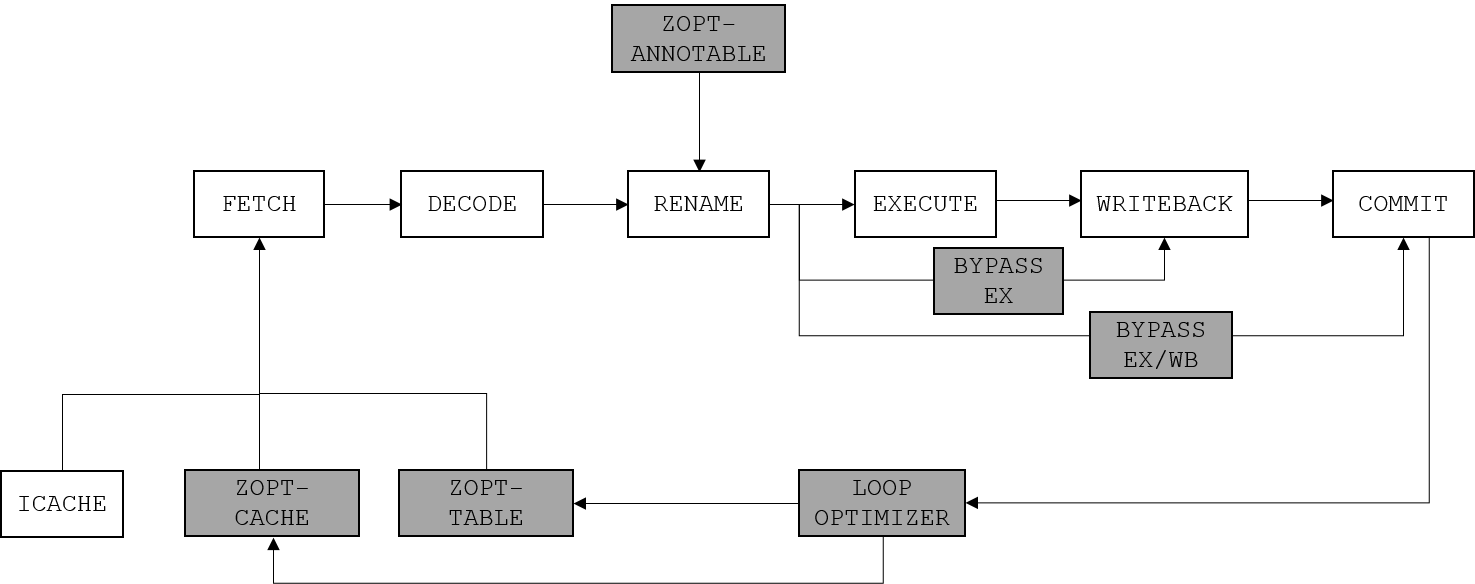
\includegraphics[height=1in]{Figures/pipeline.png}
\caption{Overview of processor extensions.}
\label{fig:opt_pipeline}
\end{figure}

\subsubsection{Front-End Extensions.}
The objectives of the front-end extensions are the following: (i) detect zero-optimizable instructions in the instruction stream and (ii) bypass pipeline stages.  These steps can be done in parallel with existing pipeline stages, as discussed below.  

\paragraph{Detect Zero-optimizable Instructions.}
This is done in the decode stage by matching the instruction opcode against a predefined set of opcodes. Since the opcode set is small, i.e., addition and multiplication opcodes, the matching can be done in parallel to avoid extra delays.  The zero-optimizable instructions detected here are marked for easy identification in later pipeline stages. 

\paragraph{Bypass Pipeline Stages.}
We exploit zero operand values to bypass the execute and writeback stages whenever possible.  This is done while a zero-optimizable instruction is in the instruction queue waiting for data dependencies.  We extend the mechanism for detecting operand availability to also check whether or not the value is zero.  For a multiplication instruction or a redundant addition instruction (i.e., destination operand is same as other source operand), we break outstanding data dependencies of the instruction making the instruction ready to issue.  We extend the issue logic to allowing issuing instructions directly to stages later than the execute stage.  This allows us to issue multiplication instructions to the writeback stage to zero the destination operand (and broadcast availability), and issue redundant additions to the commit stage.   

%Our approach performs the following operations in the pipeline front-end: (i) identify zero-optimizable instructions, (ii) detect when zero-optimizable input operand is a zero, (iii) modify producer and consumer data dependencies, and (iv) squash instructions.  These steps can be done in parallel with existing pipeline front-end stages, as we discuss below. 

%\subsubsection{Identify Zero-Optimizable Instructions.} We can detect zero-optimizable instructions during instruction decoding by matching the opcode against a predefined set of opcodes. Since only a small set of arithmetic instructions qualify as zero-optimizable, the storage requirements of the opcode set is modest, and opcode matching can be done in parallel to avoid extra delays. Zero-optimizable instructions that are identified in the decode stage are marked for easy identification in later pipeline stages. 

%\subsubsection{Detect Zero Operands.} We can detect zero input operands while a zero-optimizable instruction is waiting in the instruction queue for data dependencies.  Current mechanisms for signaling operand availability can be extended to also indicate whether or not the value is zero. 
 
 %\subsubsection{Modify Data Dependencies.}  We can extend current mechanisms for tracking data dependencies among instructions to clear dependencies of zero-optimizable instructions that become redundant due to a zero input operand becoming available. Futhermore, dependencies from instructions that consume the results of a zero-optimizable instruction should be cleared when a zero input makes the instruction an identity function, and thus redundant.  
 
 \subsubsection{Back-End Extensions.}
 Our backend extensions consists of three mechanisms: (i) detecting loops that can benefit from our optimizations, (ii) generate and cache optimized code sequences to execute in place of loops when a zero-optimizable input is zero, and (iii) switch execution to optimized code  sequences when appropriate. 
 
\paragraph{Optimizable Loop Detector} This mechanism scans the stream of committed instructions to detect loops that can be optimized based on zero-optimizable instructions. 
 
\paragraph{Loop Optimizer and Cache.}  Optimize loop based on one zero-optimizable instruction input, and cache optimized code. 
 
 \paragraph{Optimized Code Executor.} Direct control flow to optimized code sequences in place of the original code sequences.   
 
 
